% --------------------------------------------------------------------------- %
% Poster for the ECCS 2011 Conference about Elementary Dynamic Networks.      %
% --------------------------------------------------------------------------- %
% Created with Brian Amberg's LaTeX Poster Template. Please refer for the     %
% attached README.md file for the details how to compile with `pdflatex`.     %
% --------------------------------------------------------------------------- %
% $LastChangedDate:: 2011-09-11 10:57:12 +0200 (V, 11 szept. 2011)          $ %
% $LastChangedRevision:: 128                                                $ %
% $LastChangedBy:: rlegendi                                                 $ %
% $Id:: poster.tex 128 2011-09-11 08:57:12Z rlegendi                        $ %
% --------------------------------------------------------------------------- %
\documentclass[a0paper,portrait]{baposter}

\usepackage[hidelinks]{hyperref}
\usepackage{amsfonts}
\usepackage{amssymb}
\usepackage{amsmath}
\usepackage{amsbsy}
\usepackage{relsize}		% For \smaller
\usepackage{url}			% For \url
% \usepackage{epstopdf}	% Included EPS files automatically converted to PDF to include with pdflatex

%%% Global Settings %%%%%%%%%%%%%%%%%%%%%%%%%%%%%%%%%%%%%%%%%%%%%%%%%%%%%%%%%%%

\graphicspath{{pix/}}	% Root directory of the pictures 
% \tracingstats=2			% Enabled LaTeX logging with conditionals

%%% Color Definitions %%%%%%%%%%%%%%%%%%%%%%%%%%%%%%%%%%%%%%%%%%%%%%%%%%%%%%%%%

\definecolor{bordercol}{RGB}{0,0,0}
\definecolor{headercol1}{RGB}{164,52,58}
\definecolor{headercol2}{RGB}{50,50,50}
\definecolor{headerfontcol}{RGB}{0,0,0}
\definecolor{boxcolor}{RGB}{240,232,226}
\definecolor{White}{RGB}{255,255,255}

%%%%%%%%%%%%%%%%%%%%%%%%%%%%%%%%%%%%%%%%%%%%%%%%%%%%%%%%%%%%%%%%%%%%%%%%%%%%%%%%
%%% Utility functions %%%%%%%%%%%%%%%%%%%%%%%%%%%%%%%%%%%%%%%%%%%%%%%%%%%%%%%%%%

%%% Save space in lists. Use this after the opening of the list %%%%%%%%%%%%%%%%
\newcommand{\compresslist}{
	\setlength{\itemsep}{1pt}
	\setlength{\parskip}{0pt}
	\setlength{\parsep}{0pt}
}

%%%%%%%%%%%%%%%%%%%%%%%%%%%%%%%%%%%%%%%%%%%%%%%%%%%%%%%%%%%%%%%%%%%%%%%%%%%%%%%
%%% Document Start %%%%%%%%%%%%%%%%%%%%%%%%%%%%%%%%%%%%%%%%%%%%%%%%%%%%%%%%%%%%
%%%%%%%%%%%%%%%%%%%%%%%%%%%%%%%%%%%%%%%%%%%%%%%%%%%%%%%%%%%%%%%%%%%%%%%%%%%%%%%
\begin{document}

\typeout{Poster rendering started}

%%% Setting Background Image %%%%%%%%%%%%%%%%%%%%%%%%%%%%%%%%%%%%%%%%%%%%%%%%%%
\background{
	\begin{tikzpicture}[remember picture,overlay]%
	\draw (current page.north west)+(-2em,2em) node[anchor=north west]
	{
\includegraphics[height=1.1\textheight]{Capturas y gráficos/WhiteToRed.png}};
	\end{tikzpicture}
}

%%% General Poster Settings %%%%%%%%%%%%%%%%%%%%%%%%%%%%%%%%%%%%%%%%%%%%%%%%%%%
%%%%%% Eye Catcher, Title, Authors and University Images %%%%%%%%%%%%%%%%%%%%%%
\begin{poster}{
	grid=false,
	% Option is left on true though the eyecatcher is not used. The reason is
	% that we have a bit nicer looking title and author formatting in the headercol
	% this way
	%eyecatcher=false, 
	borderColor=bordercol,
	headerColorOne=headercol1,
	headerColorTwo=headercol2,
	headerFontColor=headerfontcol,
	% Only simple background color used, no shading, so boxColorTwo isn't necessary
	boxColorOne=boxcolor,
	headershape=roundedright,
	headerfont=\Large\sf\bf,
	textborder=rectangle,
	background=user,
	headerborder=open,
  boxshade=plain
}
%%% Eye Cacther %%%%%%%%%%%%%%%%%%%%%%%%%%%%%%%%%%%%%%%%%%%%%%%%%%%%%%%%%%%%%%%
{
	Eye Catcher, empty if option eyecatcher=false - unused
}
%%% Title %%%%%%%%%%%%%%%%%%%%%%%%%%%%%%%%%%%%%%%%%%%%%%%%%%%%%%%%%%%%%%%%%%%%%
{\sf\bf \scshape
\vspace{-4mm}
	C\hspace{1mm}a\hspace{1mm}r\hspace{1mm}g\hspace{1mm}a\hspace{1mm}s\hspace{3mm} E\hspace{1mm}l\hspace{1mm}e\hspace{1mm}c\hspace{1mm}t\hspace{1mm}r\hspace{1mm}o\hspace{1mm}s\hspace{1mm}t\hspace{1mm}á\hspace{1mm}t\hspace{1mm}i\hspace{1mm}c\hspace{1mm}a\hspace{1mm}s
}
%%% Authors %%%%%%%%%%%%%%%%%%%%%%%%%%%%%%%%%%%%%%%%%%%%%%%%%%%%%%%%%%%%%%%%%%%
{
	\vspace{1em} A. D. Hernández-Melo$^\heartsuit$, E. S. Pulido-Reyes$^\diamondsuit$, y A. A. Santoyo-Noeggerath$^\dagger$ \\
	{\smaller $^\heartsuit$he312453@uaeh.edu.mx, $^\diamondsuit$pu359528@uaeh.edu.mx, $^\dagger$sa352740@uaeh.edu.mx}\\ \vspace{2mm}
	{\footnotesize $^\heartsuit$$^\diamondsuit$$^\dagger${Área Académica de Matemáticas y Física, Instituto de Ciencias Básicas e Ingenierías, Universidad Autónoma del Estado} \par} 
	{\footnotesize {de Hidalgo, Carretera Pachuca-Tulancingo Km. 4.5, Col. Carboneras, C.P. 42184, Mineral de la Reforma, Hidalgo, México} \par}
}
%%% Logo %%%%%%%%%%%%%%%%%%%%%%%%%%%%%%%%%%%%%%%%%%%%%%%%%%%%%%%%%%%%%%%%%%%%%%
{
% The logos are compressed a bit into a simple box to make them smaller on the result
% (Wasn't able to find any bigger of them.)
\setlength\fboxsep{0pt}
\setlength\fboxrule{0pt}
	\fbox{
		\begin{minipage}{17em}
			\href{https://www.uaeh.edu.mx/}{
\includegraphics[scale=0.26]{Capturas y gráficos/UAEH Logo.png}}
		\end{minipage}
	}
}

\headerbox{\textcolor{White}{Resumen}}{name=problem,column=0,row=0}{
Con ayuda del software \textit{PhET} se experimentara con un par de cargas eléctricas y la relación que tienen con la ley de Coulomb, así mismo se podrá variar la distancia en que las cargas se ubican y/o la carga eléctrica de cada carga para observar que es lo que pasa con la fuerza eléctrica calculada y al final observar como cambia la ley de Coulomb. \par
\vspace{2mm}
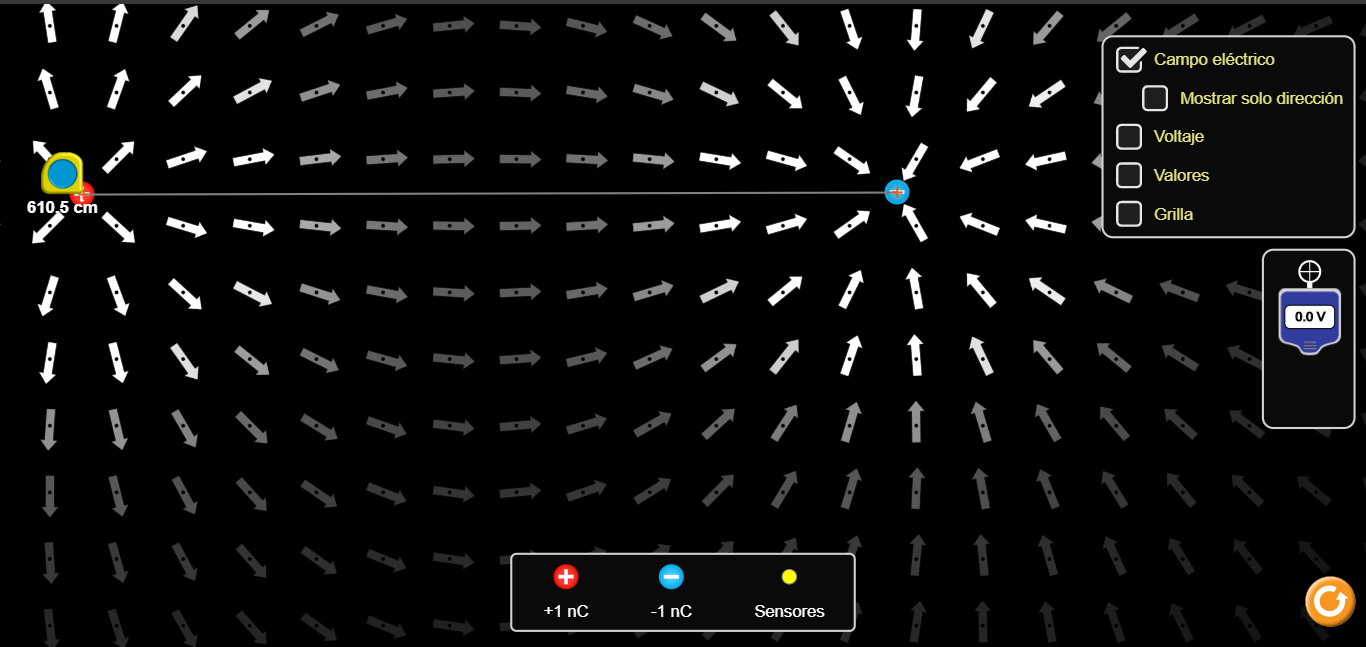
\includegraphics[width=\linewidth]{Capturas y gráficos/Captura1.PNG}
}

\headerbox{\textcolor{White}{ Introducción}}{name=definitions,column=0,below=problem}{
La fuerza electromagnética es una de las clases de las fuerzas fundamentales. Este tipo de interacciones supone que las partículas tienen una propiedad conocida como \textit{carga eléctrica}, y se rigen por la \textit{Ley de Coulomb}:\par
\vspace{-2mm}
\begin{center}
$F=\dfrac{1}{4\pi \epsilon_0}\dfrac{|qq_0|}{r^2}$\par
\end{center} 
\vspace{-2mm}
Las fuerzas electromagnéticas se dividen en dos: Fuerza de Atracción y Fuerza de Repulsión, se dirá que en un sistema actúa una u otra fuerza dependiendo del valor de las cargas que interactúen.
}

\headerbox{\textcolor{White}{Métodos Experimentales}}{name=models,column=0,below=definitions}
{Con apoyo del software "PhET" se midió como interactúan las fuerzas eléctricas dependiendo la distancia y la magnitud de las cargas empleadas así como su signo, aunado a esto también existe la oportunidad de cambiar de escala, entre una escala macro (que en principio es más fácil de comprender) a una atómica (con valores que incluyen exponentes aproximadamente de micro unidades), a lo largo de esta practica se vario la distancia, magnitud y signo de las cargar eléctricas empleadas para observar como afecta esto al resultado de la fuerza eléctrica.
}

\headerbox{\textcolor{White}{ Referencias}}{name=references,column=0,below=models}{
\smaller										% Make the whole text smaller
\vspace{-0.4em} 										% Save some space at the beginning
\bibliographystyle{plain}							% Use plain style
\renewcommand{\section}[2]{\vskip 0.05em}		% Omit "References" title
\begin{thebibliography}{1}							% Simple bibliography with widest label of 1
\itemsep=-0.01em										% Save space between the separation
\setlength{\baselineskip}{0.4em}					% Save space with longer lines
\bibitem{1}{R.A. Serway, J.W. Jewett Jr., Física para Ciencias e Ingeniería con Física Moderna, séptima edición, Cengage Learning, México, 2009.} \par
\bibitem{2}{H.D. Young, Y. Freedman, Física Universitaria con Física Moderna, décimo tercera edición, PEARSON, México, 2013.} \par
\bibitem{3}{D. Halliday, R. Resnick, \& K.S. Krane, Física Volumen 2, cuarta edición, Editorial Continental, México, 1999.} \par
\bibitem{4}{D. Giancoli, Física para Ciencias e Ingenierías. Volumen 2, Cuarta edición, PEARSON, México, 2009} \par
\bibitem{5}{Ley de Coulomb. PhET: Interactive Simulations. \\ https://phet.colorado.edu/sims/html/coulombs-law/latest/coulombs-law\_es.html. \\ 2020 (Accessed 21 August 2020)} \par
\end{thebibliography}
}

\headerbox{\textcolor{White}{\smaller Agradecimientos}}{name=acknowledgements,column=0,below=references, above=bottom}{
{
\smaller\footnotesize				% Make the whole text smaller
\vspace{-0em}			% Save some space at the beginning
Agradecemos al doctor Mario Pérez González por brindarnos apoyo académico para realizar esta practica así como a los doctores y expertos de la \textit{University of Colorado Boulder} por la utilización del software \textit{PhET}. \par
}
} 

\headerbox{\textcolor{White}{Resultados y Discusiones}}{name=density,span=2,column=1,row=0}{
Gracias a que el software \textit{PhET} es una simulación con base a la ley de coulomb,  los distintos datos recolectados en la simulación entonces siguen con perfección la tendencia. Como es de esperarse, si se analizan las dos primeras gráficas, se observa que la fuerza eléctrica disminuye con una forma cuadrática al aumentar la distancia y de forma análoga con la carga negativa, de tal modo que la conjunción de ambas es simétrica conforme al eje x en $y = 0$
en los dos casos de escala (macro y atómica). ya que en la escala atómica las distancias capturadas crecen mas rápidamente a comparación de las distancias capturadas en las gráficas a macro escala, se puede observar un salto en la fuerza eléctrica, esto es solo una falta de datos entre la primer y segunda toma  de ellos. obteniendo así dos gráficas análogas a las macroscópicas. Con respecto al error obtenido, se puede observar que es mayor al inicio, cuando la distancia entre las cargas es pequeña, con alrededor de un 1.7\% cual es suficientemente pequeño para decir que es bueno. 
\vspace{-1em}
\begin{center}
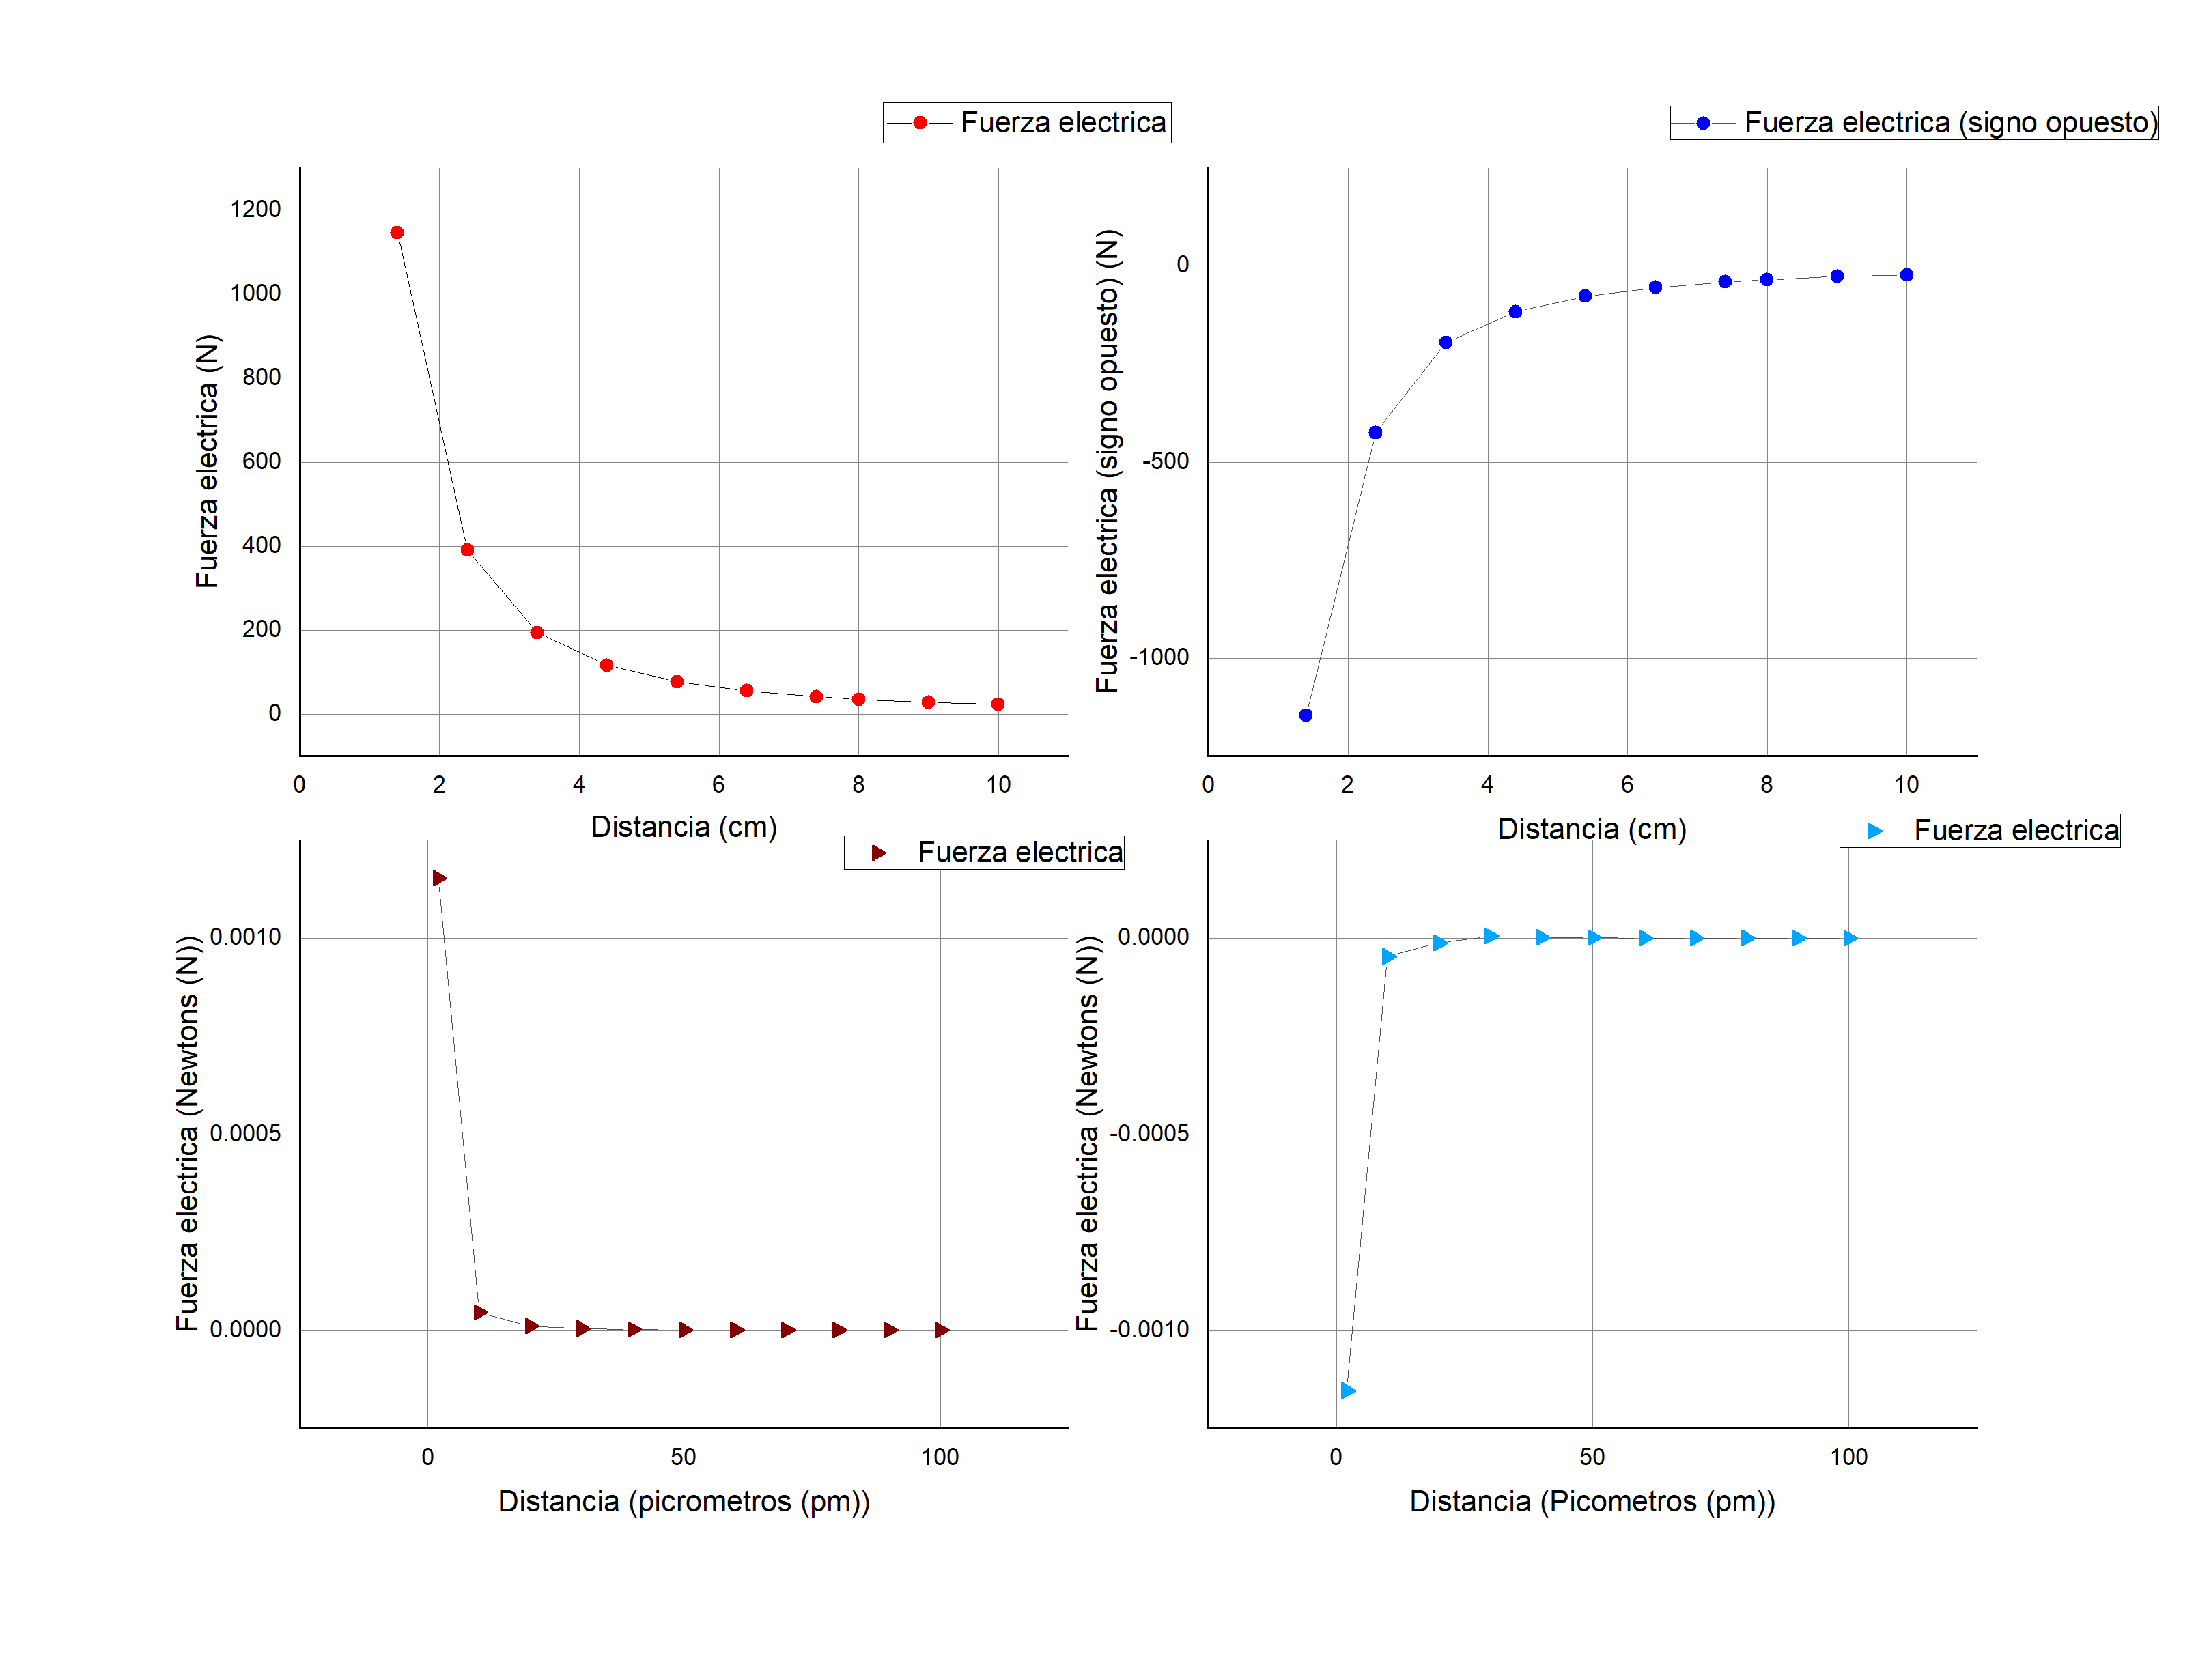
\includegraphics[angle=0,width=1\linewidth]{Capturas y gráficos/Graficosye.png}
\end{center}
\vspace{-4.6em}
\begin{center}
	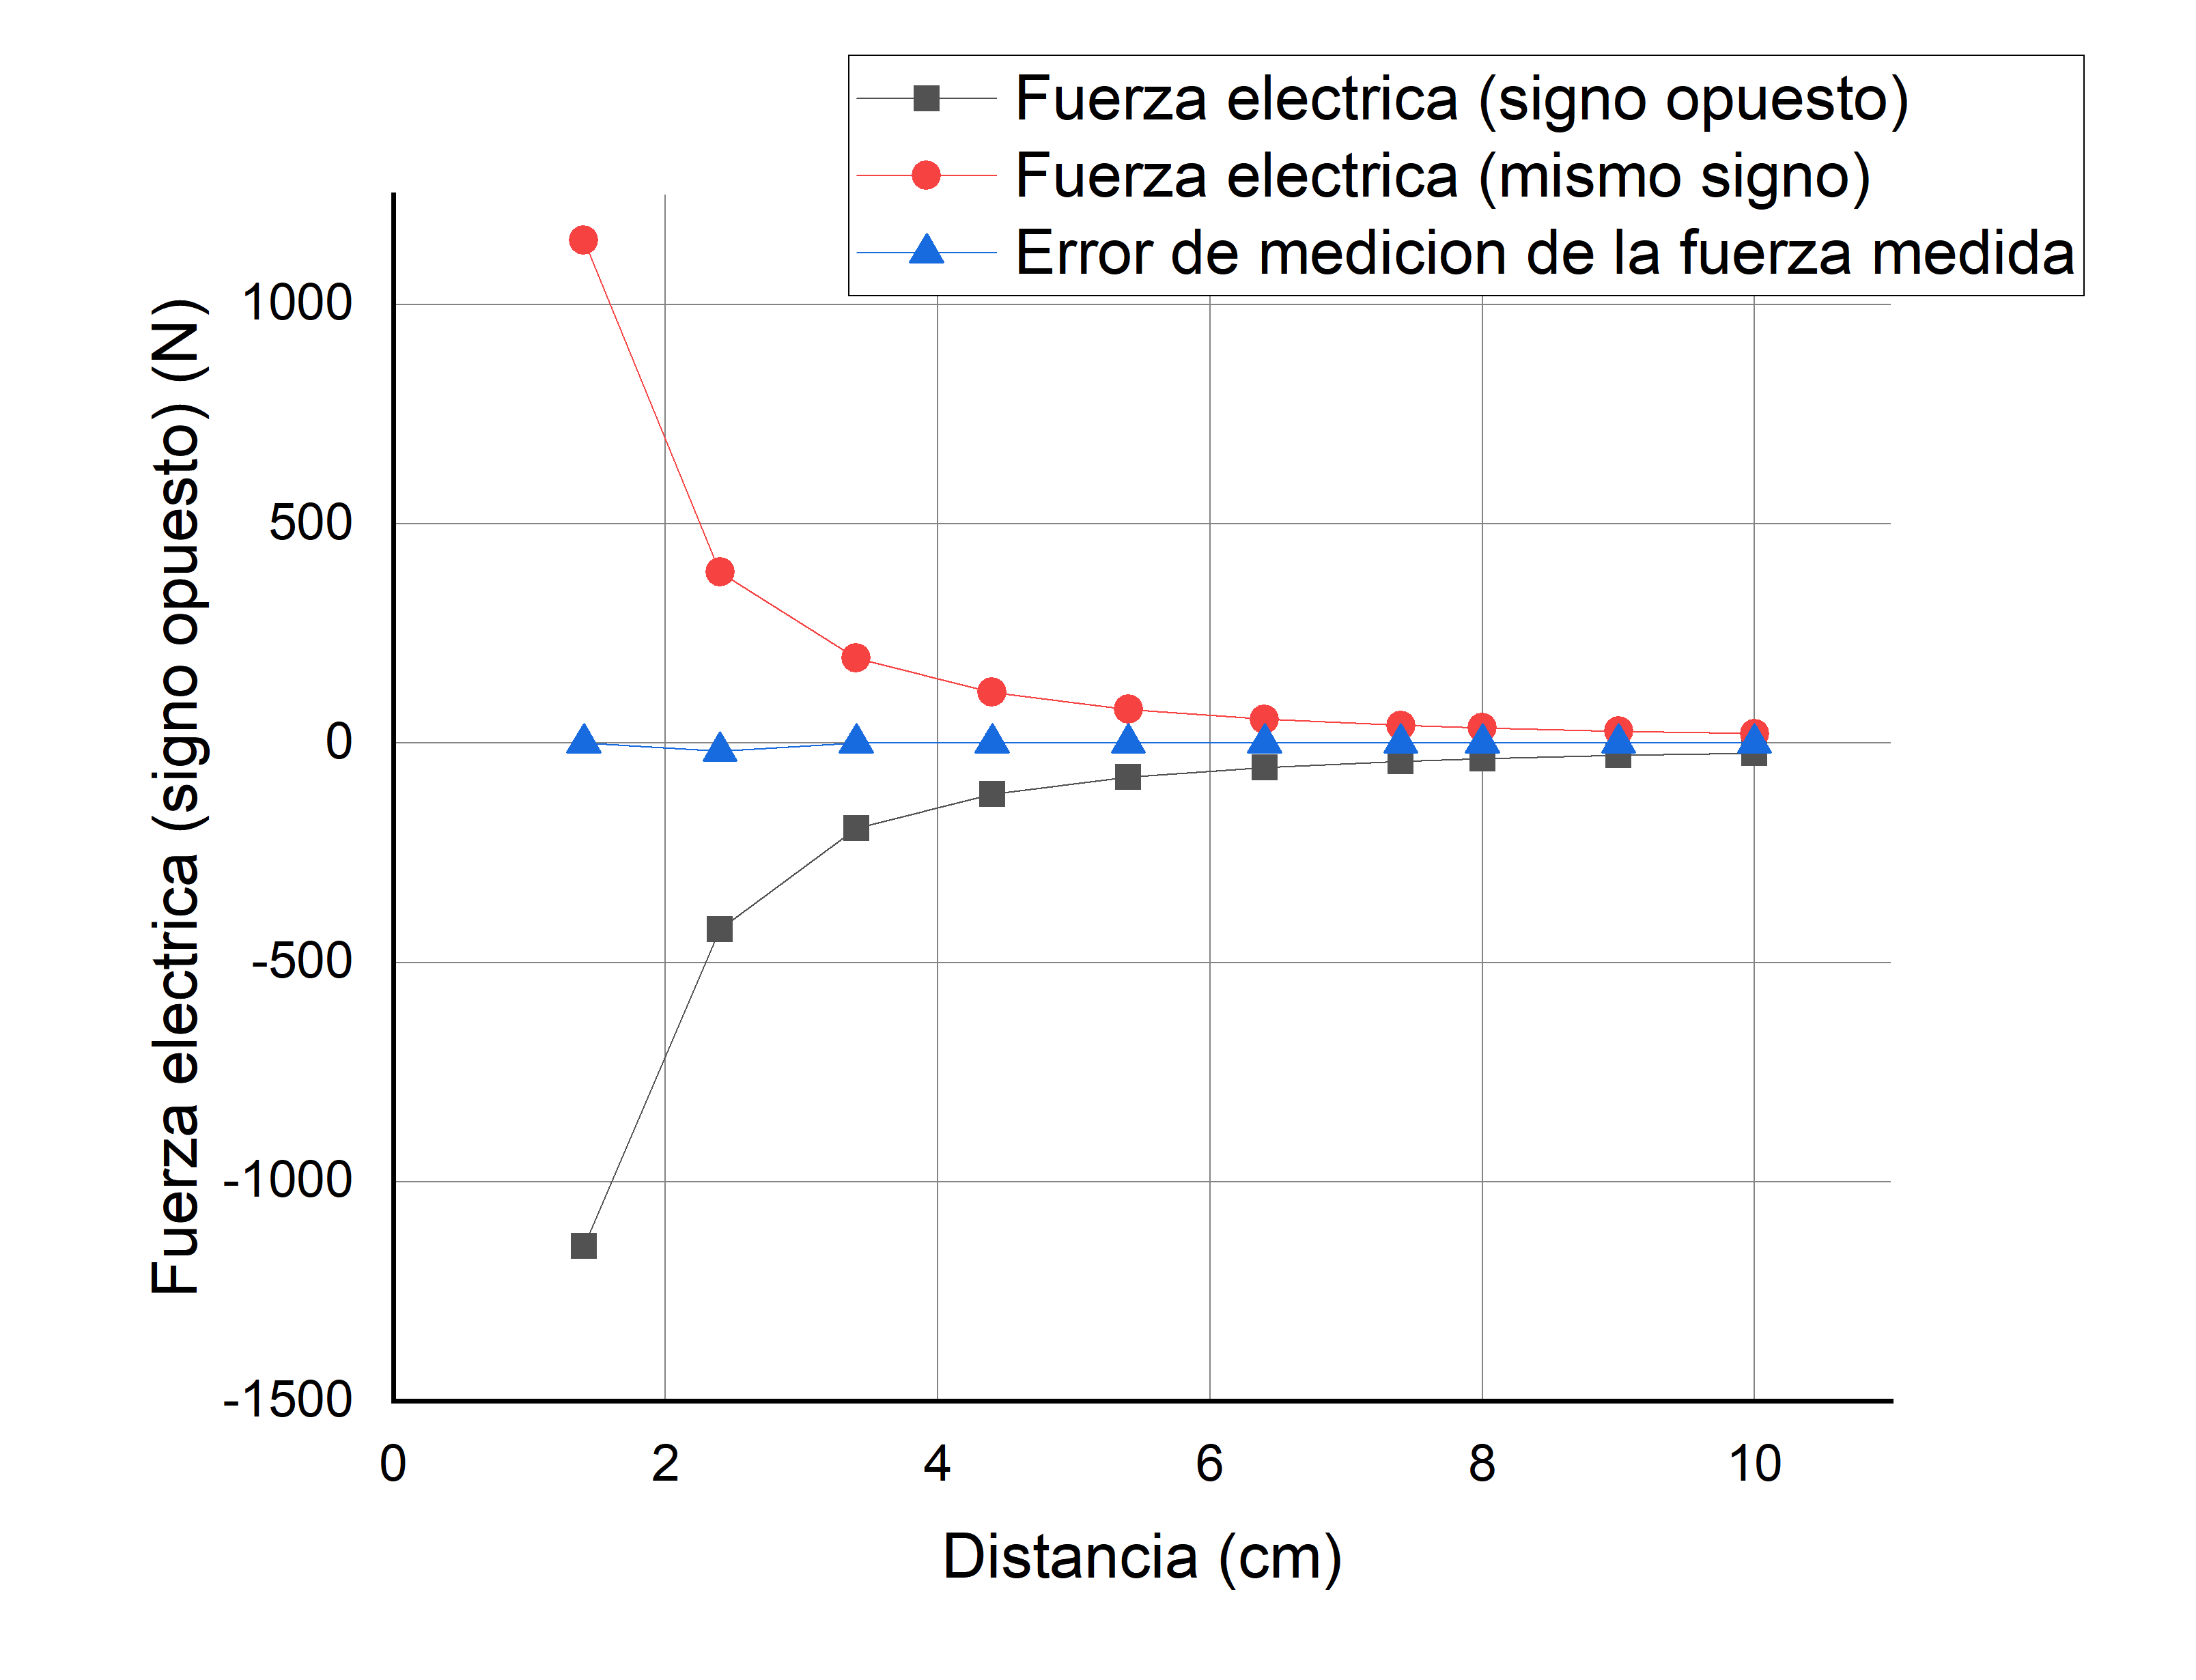
\includegraphics[angle=0,width=0.49\linewidth]{Capturas y gráficos/Graph3cargas_ye.png} \hspace{-3em}
	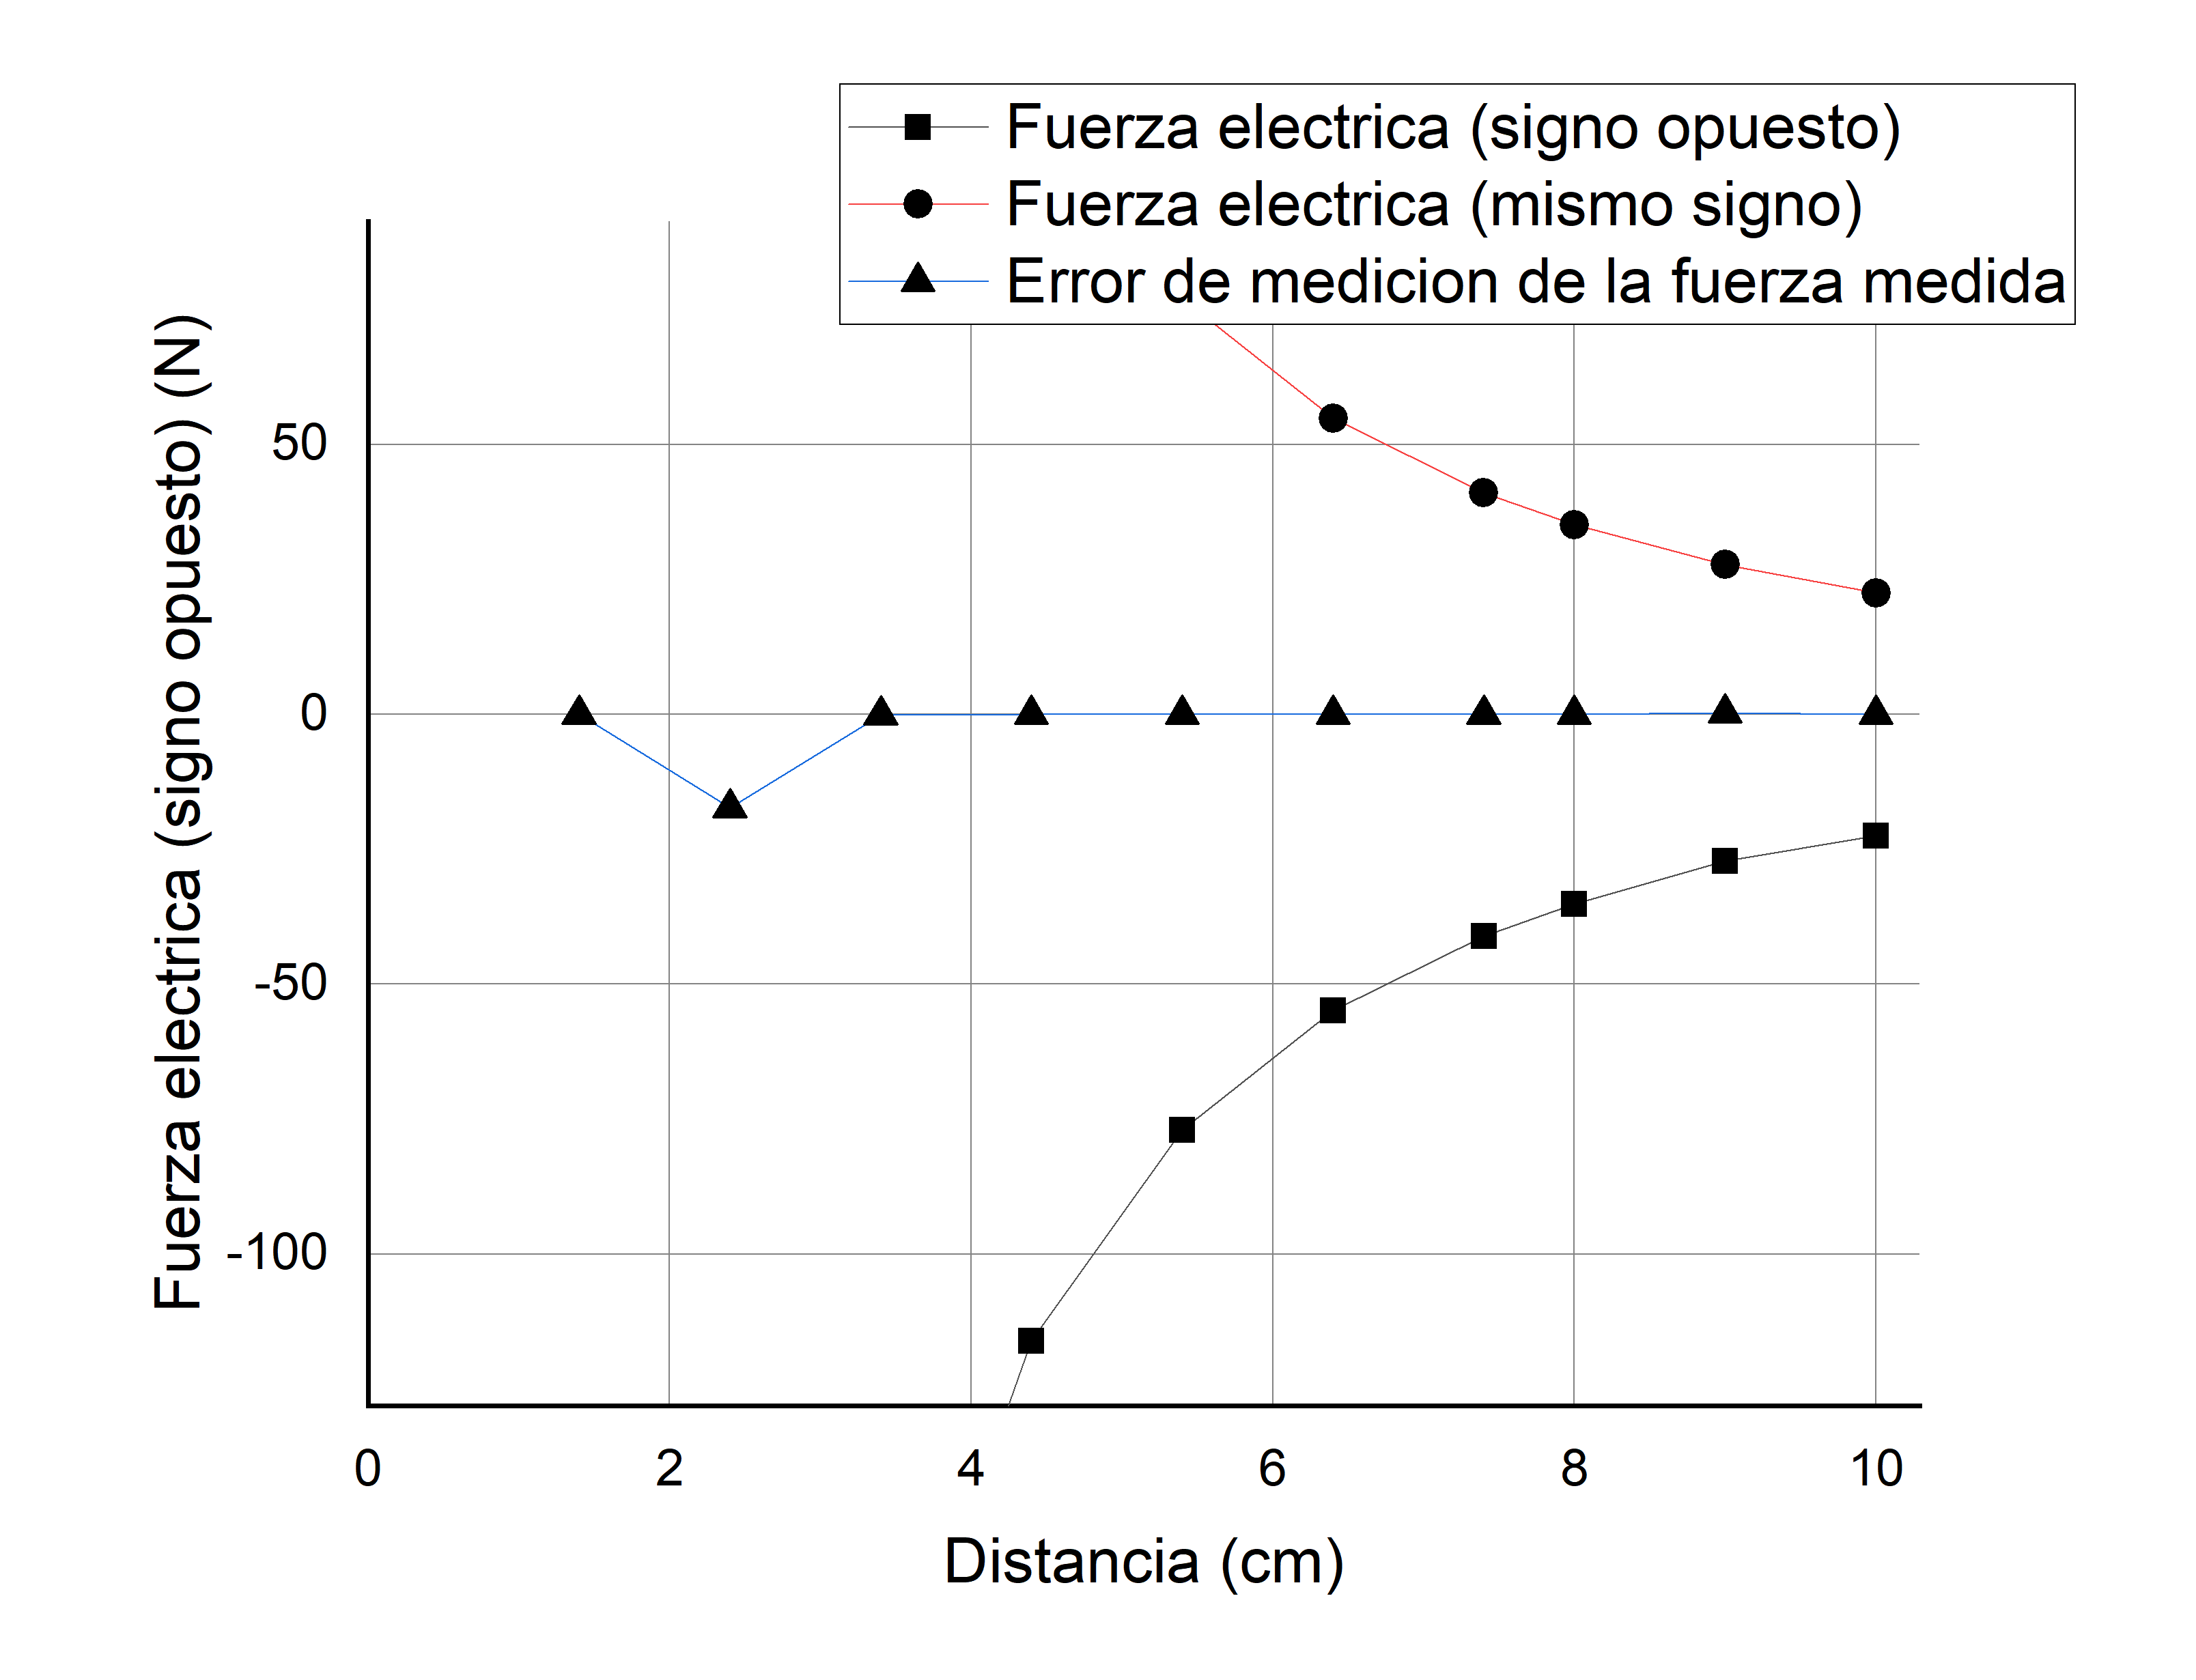
\includegraphics[angle=0,width=0.49\linewidth]{Capturas y gráficos/Graph3.1_ye.png}
\end{center}
\vspace{0.5em}
}

\headerbox{\textcolor{White}{Conclusiones}}
{name=degreeDistribution,span=2,column=1,below=density,above=bottom}{
Con el apoyo de la simulación es fácil comprender físicamente lo que  sucede al dos cargas acercarse una a la otra. Cuando las cargas en cuestión son de signo igual, entonces los vectores de fuerza apuntan en dirección opuesta a la otra carga y de forma contraria cuando las cargas son de signos opuestos, los vectores de fuerza entre ellos apuntan en dirección a la otra carga, entonces se atraen mutuamente, esta fuerza ya mencionada decrece con $1/r^2$ con r siendo la distancia entre ellas, y se puede observar que de la misma forma sucede en la escala macroscópica así como en la escala atómica. El conocimiento a profundidad de lo que es la ley de coulomb es crucial para comprensión de los siguientes materiales de trabajo en electricidad y magnetismo ya que es una base grande para muchos fenómenos más complejos y conceptos mas abstractos en conjunto con la teor
ía matematica que los acompaña. 
\vspace{-0.2em}

}

\end{poster}
\end{document}
